\section{Tipos de sensores}
\textbf{Por posición:}

\textbf{Encoder Incremental:} Este tipo de sensor óptico digital convierte el movimiento en una secuencia de pulsos digitales. Tiene una escala transparente con una retícula opaca; de un lado, tiene una escala equipada con una fuente de luz y un lente condensador. Del otro lado, hay celdas sensibles a la luz. La manera en la que funciona es que la resistencia de las celdas disminuye cada vez que reciben un rayo de luz, de este modo se genera un pulso cada vez que un rayo de luz es atravesado.\autoref{fig:20150317193931229}

considerable.\autoref{fig:lvdt} \\
\begin{figure}[h]
	\centering
	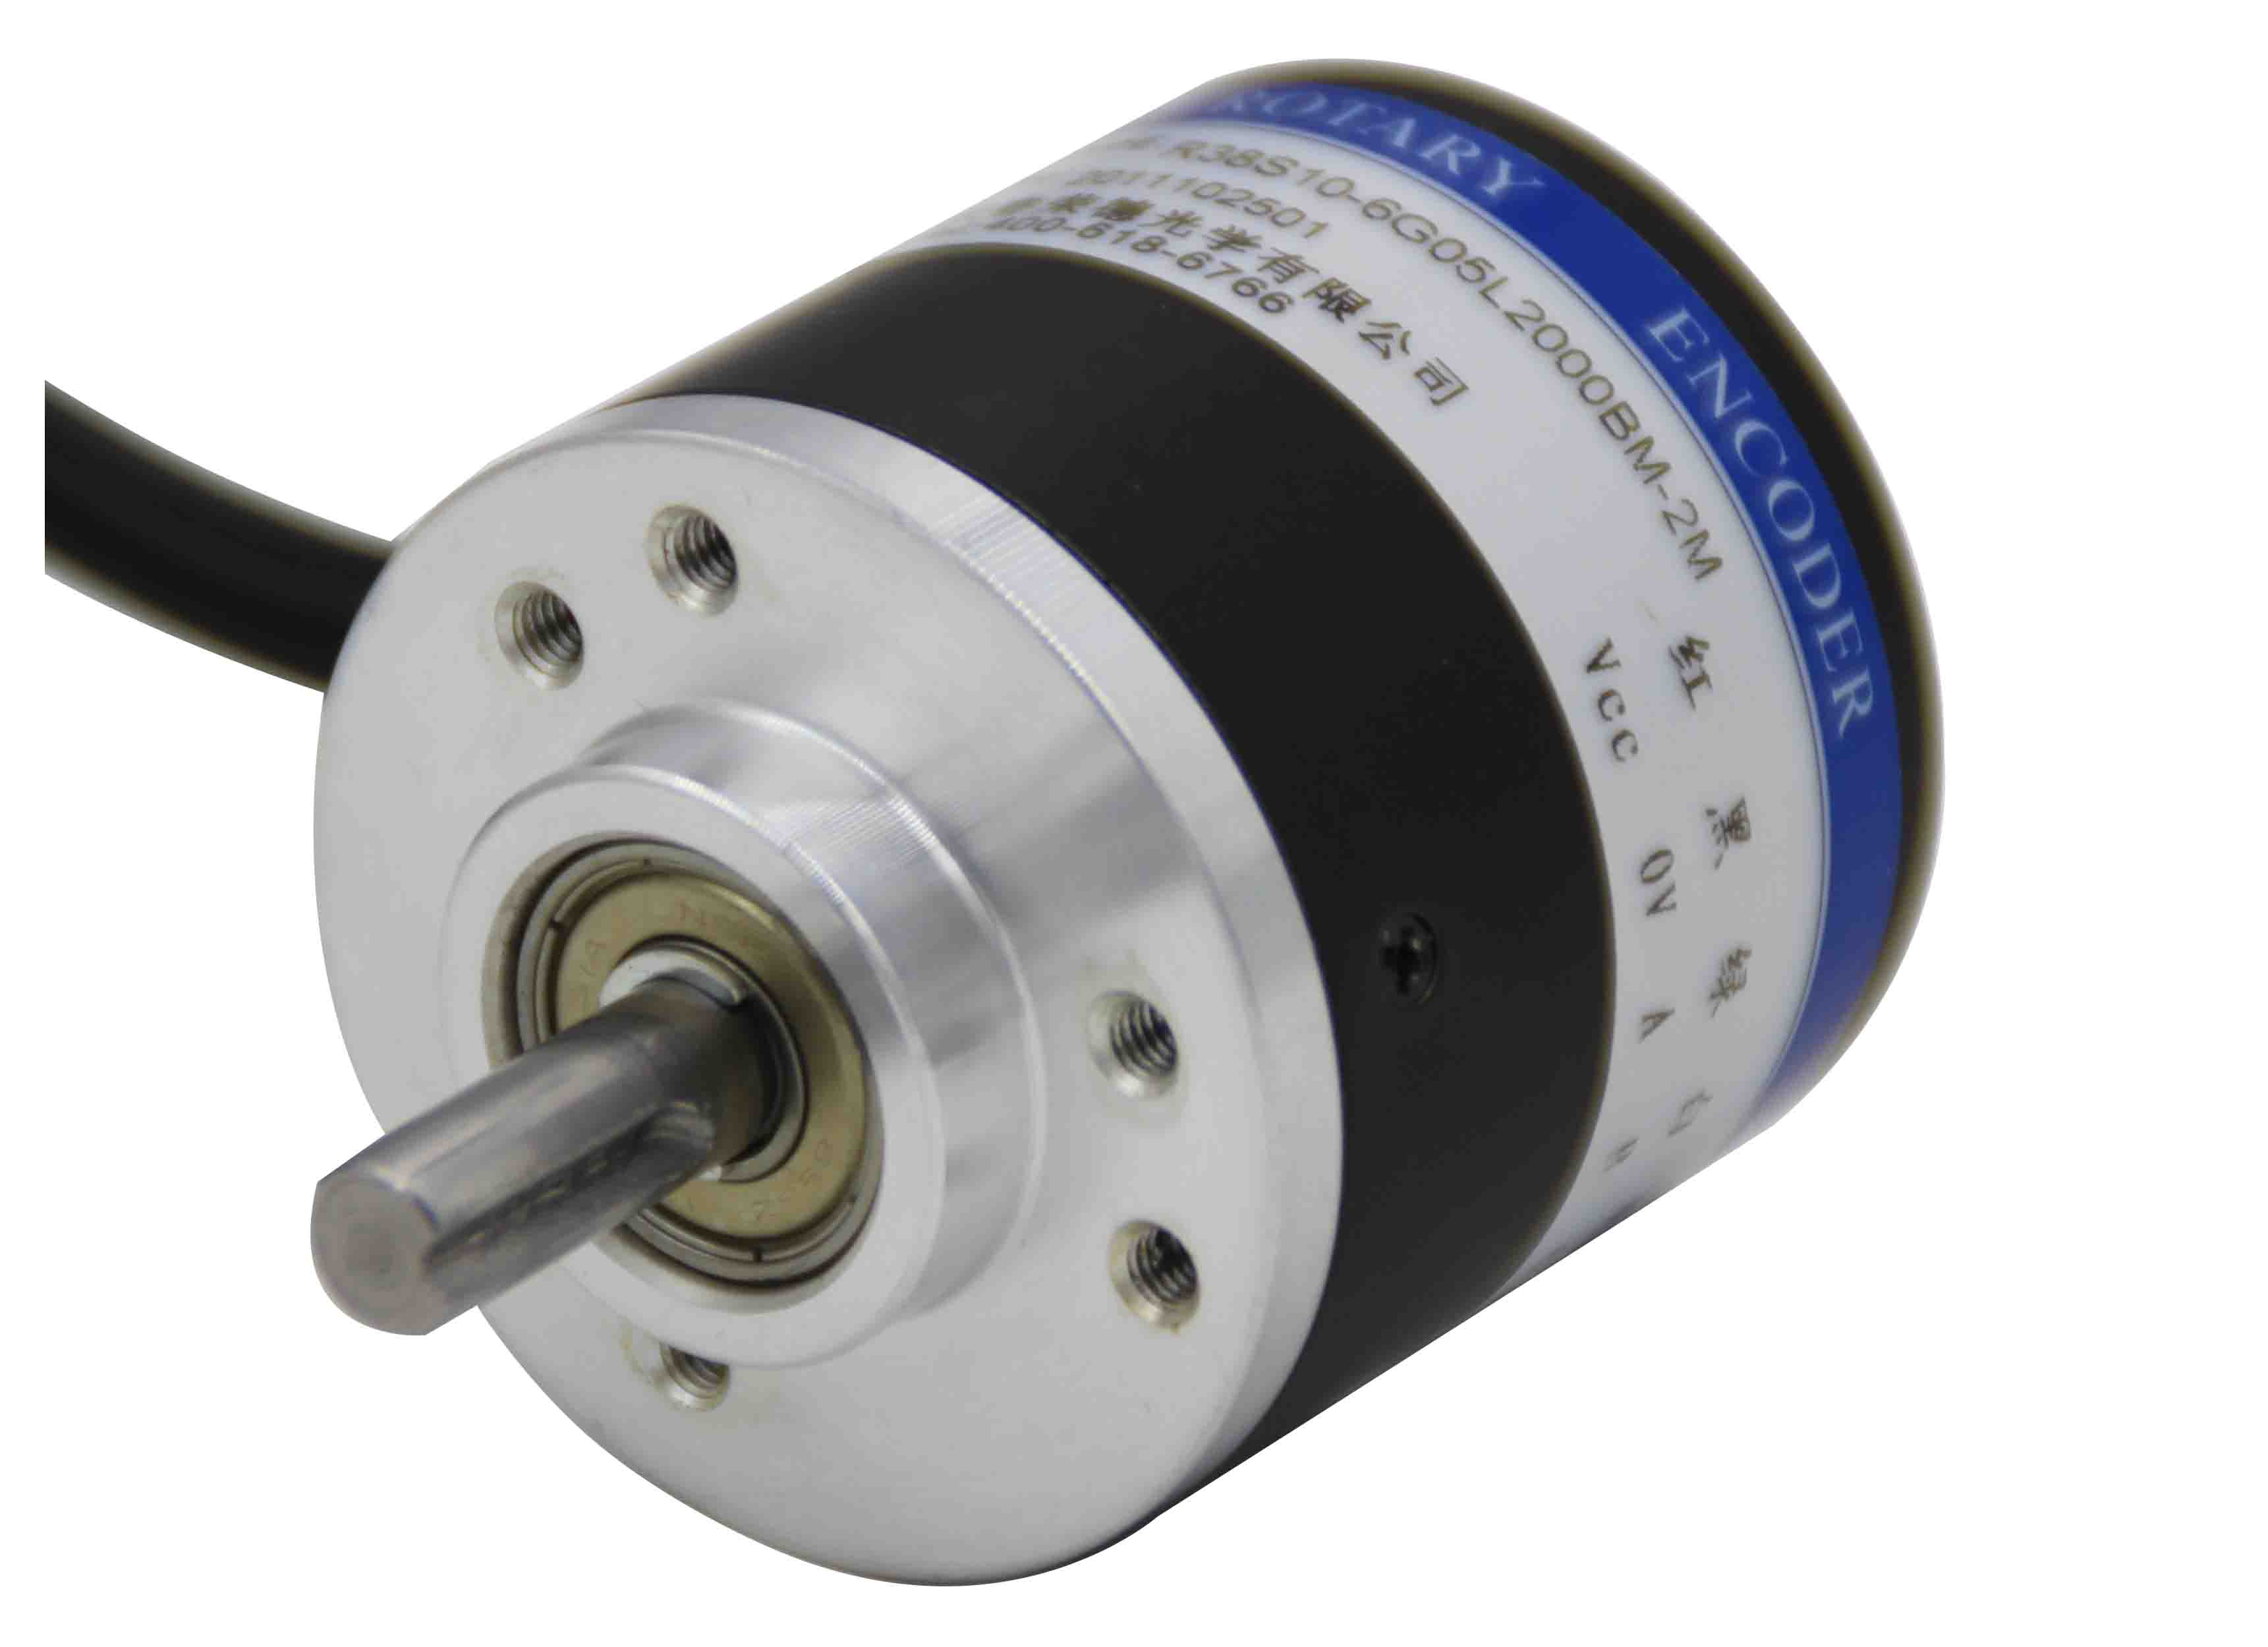
\includegraphics[width=0.4\linewidth]{portada/20150317193931229}
	\caption{}
	\label{fig:20150317193931229}
\end{figure}

\textbf{Potenciómetro:} Es un dispositivo de resistencia variable que expresa desplazamientos lineales o angulares en términos de voltaje. Consiste en una clavija deslizante que hace contacto con un elemento resistivo, conforme se mueve este punto de contacto la resistencia entre el contacto deslizante y las conexiones de los extremos del dispositivos cambia en proporción al desplazamiento. \autoref{fig:potenciometro}\\\\\\\\\\\\\\\\\\

\begin{figure}[h]
	\centering
	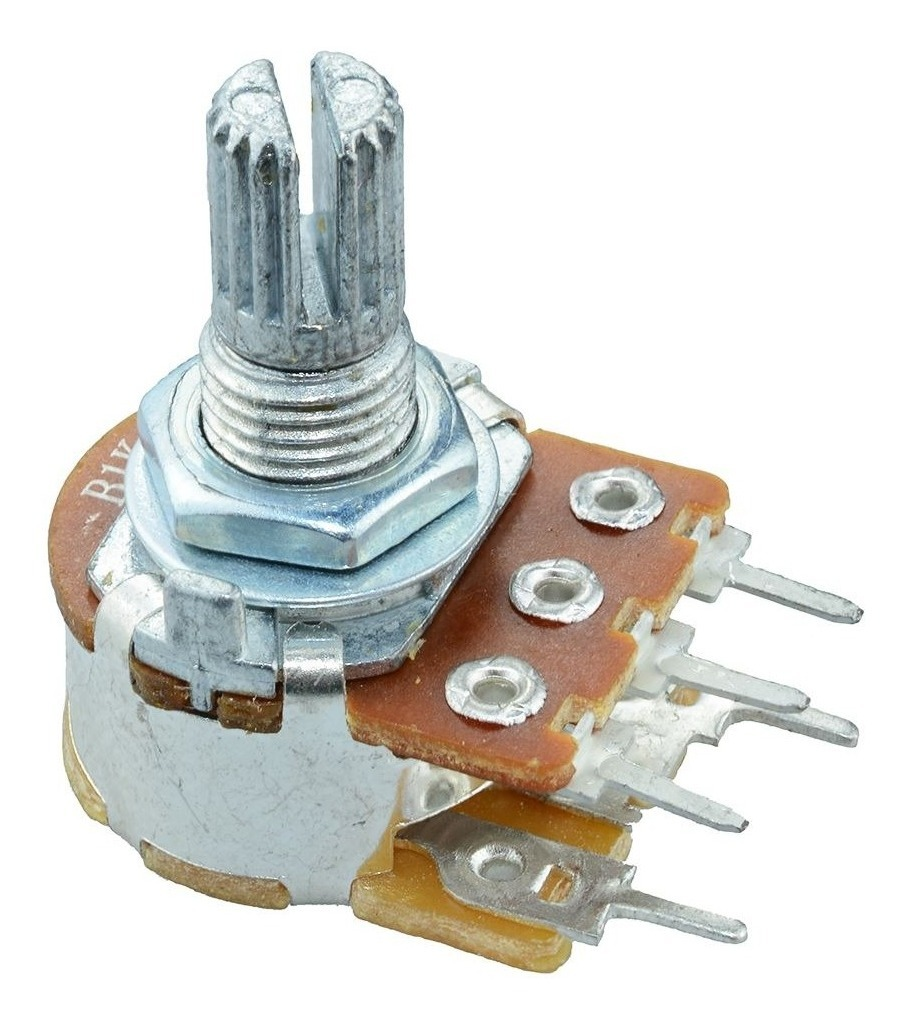
\includegraphics[width=0.2\linewidth, height=0.2\textheight]{img/potenciometro}
	\caption[Potenciómetro]{}
	\label{fig:potenciometro}
\end{figure}



\textbf{LVDT:} Es uno de los transductores de desplazamiento más populares ya que genera una señal de CA cuya magnitud se relaciona con el desplazamiento de un núcleo móvil. Tiene como concepto básico de un núcleo móvil rodeado por dos bobinas secundarias y una bobina principal y conforme el núcleo cambia su posición con respecto a las bobinas cambia también el campo magnético y por tanto se modifica la amplitud de voltaje en la bobina secundaria como una función del desplazamiento del núcleo a través de un segmento 



\begin{figure}[h]
	\centering
	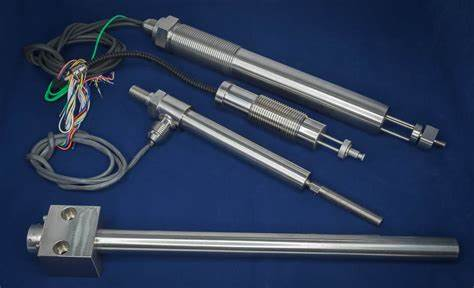
\includegraphics[width=0.2\linewidth, height=0.2\textheight]{img/LVDT}
	\caption{}
	\label{fig:lvdt}
\end{figure}




\textbf{Resolver:} Son sensores que proporcionan señales análogas como salidas y consisten en un eje (flecha) giratoria (rotor) y una carcasa estacionaria. Sus señales tienen que convertirse a la forma digital por medio de un convertidor analógico a digital. Los resólvers tienen dos devanados orientados a 90°. \autoref{fig:resolver}

\begin{figure}[!]
	\centering
	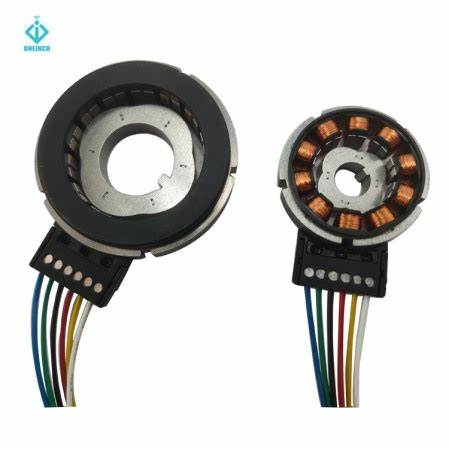
\includegraphics[width=0.2\linewidth, height=0.15\textheight]{img/resolver}
	\caption[Resolver]{}
	\label{fig:resolver}
\end{figure}




\textbf{Velocidad-tacogeneratriz :}

La captación de la velocidad se hace necesaria para mejorar el comportamiento dinámico de los actuadores del robot. La velocidad de movimiento de cada actuador (que tras el reductor es la velocidad de la articulación) se realimenta normalmente a un bucle de control analógico implementado en el propio accionador del elemento motor. No obstante, en ocasiones en las que el sistema de control del robot lo exija, la velocidad de giro de cada actuador es llevada hasta la unidad de control del robot. Normalmente, y puesto que el bucle de control de velocidad es analógico, el captador usado es una tacogeneratriz que proporciona una tensión proporcional a la velocidad de giro de su eje (valores típicos pueden ser 10 milivoltios por rpm). Otra posibilidad, usada para el caso de que la unidad de control del robot precise valorar la velocidad de giro de las articulaciones, consiste en derivar la información de posición que ésta posee.\autoref{fig:oip}



\begin{figure}[h]
	\centering
	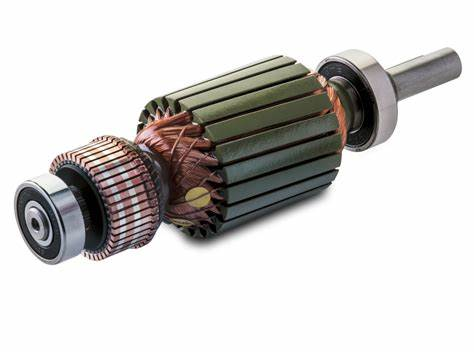
\includegraphics[width=0.2\linewidth, height=0.2\textheight]{img/OIP}
	\caption{}
	\label{fig:oip}
\end{figure}

\textbf{Tacometro:}

Estos sensores pueden encontrar directamente la velocidad en cualquier momento ya que estos miden la velocidad de rotación de un elemento. Su diseño se basa en la regla de Fleming que declara que “el voltaje producido es proporcional al índice del acoplamiento inductivo”. Aquí un conductor (básicamente una bobina) se sujeta al elemento rotativo que gira en un campo magnético (estator). Conforme incrementa la velocidad del eje, el voltaje producido en las terminales de las bobinas también aumenta.\autoref{fig:tacometro}


\begin{figure}[h]
	\centering
	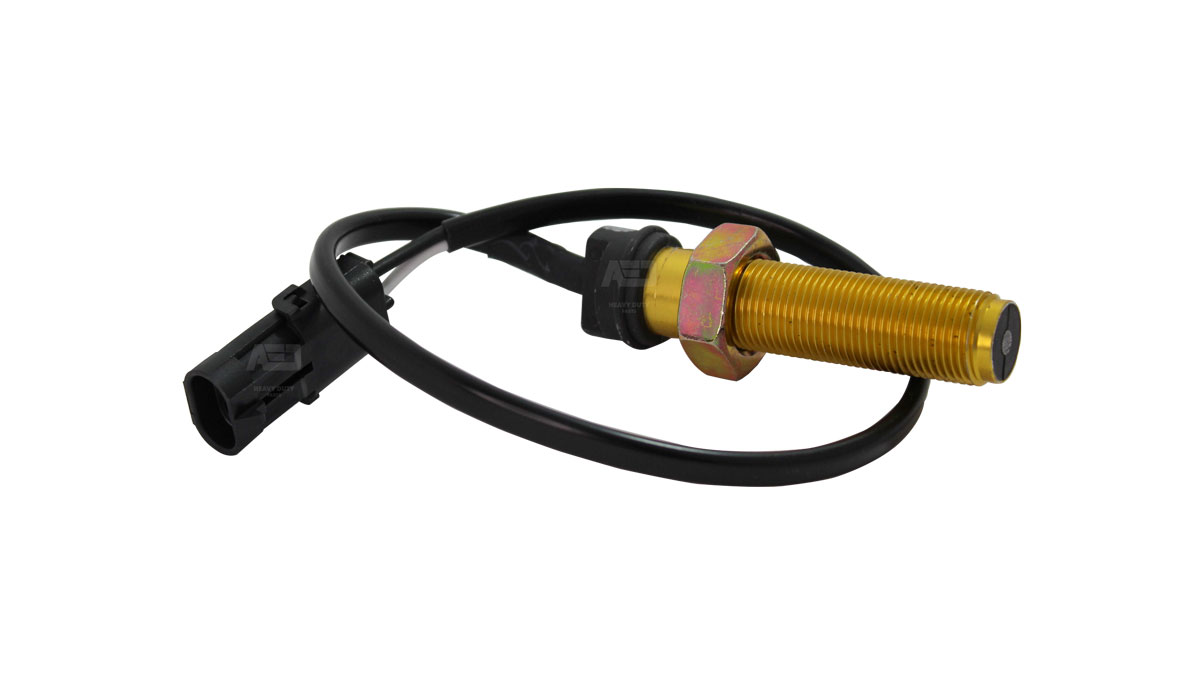
\includegraphics[width=0.5\linewidth, height=0.3\textheight]{img/tacometro}
	\caption[Tacometro]{}
	\label{fig:tacometro}
\end{figure}

\textbf{Sensor de Efecto Hall:}

Es un sensor de medición de velocidad el cual tiene el principio de “Si una pieza plana de material conductivo llamada chip Hall se sujeta a una diferencia de potencial en sus dos lados opuestos entonces el voltaje que se genera a través de las caras perpendiculares es cero”.\autoref{fig:hall}\\\\\\\\\\


\begin{figure}[h]
	\centering
	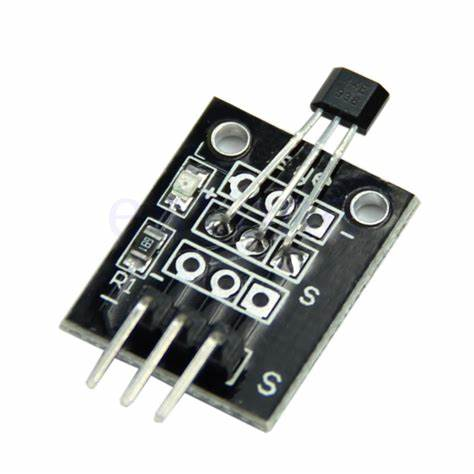
\includegraphics[width=0.2\linewidth, height=0.2\textheight]{img/HALL}
	\caption{}
	\label{fig:hall}
\end{figure}




\textbf{Galgas extensométricas:}

El principio de este sensor es que el alargamiento de un conductor aumenta su resistencia eléctrica. Este incremento de resistencia se debe a incremento de la longitud del conductor y decremento en el área del conductor.\autoref{fig:galga-extensiometrica-300x202}

\begin{figure}[h]
	\centering
	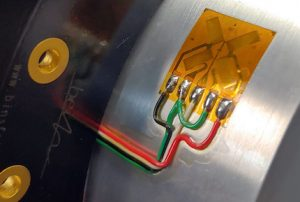
\includegraphics[width=0.3\linewidth, height=0.2\textheight]{img/galga-extensiometrica-300x202}
	\caption{}
	\label{fig:galga-extensiometrica-300x202}
\end{figure}

\textbf{Interruptores piezoeléctricos:}

Son sensores que utilizan un material piezoeléctrico el cual señala que cuando cristales eléctricos asimétricos se deforman mediante una fuerza, se desarrolla un potencial eléctrico dentro de la red cristalina deformada. Son capaces de medir fuerzas, presiones, vibraciones y aceleraciones.\\\\\\\\\\\\


\begin{figure}[h]
	\centering
	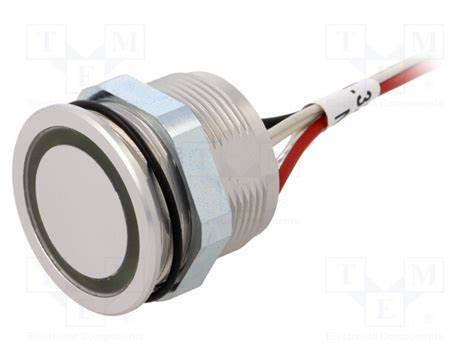
\includegraphics[width=0.3\linewidth, height=0.2\textheight]{img/S}
	\caption[f]{}
	\label{fig:s}
\end{figure}

\textbf{Tipo de contacto: }

\textbf{Interruptores de límite: }
Un interruptor de límite tiene un brazo mecánico sensible a la presión, y al momento  en el que un  objeto aplica presión en el brazo, se activa el interruptor.  Contiene un mecanismo de conmutación el cual su actuador activa el mecanismo que cierra o abre un circuito eléctrico. 
\begin{figure}[h]
	\centering
	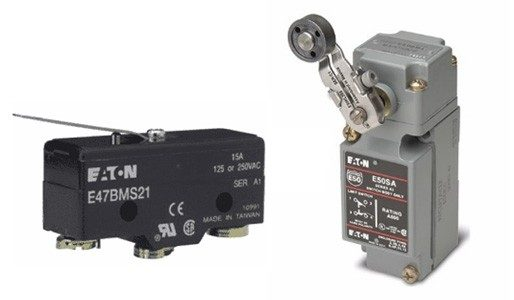
\includegraphics[width=0.4\linewidth, height=0.2\textwidth]{img/intlimite}
	\caption{}
	\label{fig:intlimite}
\end{figure}

\textbf{Interruptores neumáticos: }
Son un tipo de dispositivo de conmutación que utiliza aire para funcionar. Al momento que se comprime el interruptor neumático envía un soplo a lo largo del tubo de PCV y llega a un interruptor de aire. El movimiento del aire activará el interruptor de aire, que creará el circuito eléctrico y activará un dispositivo.
\begin{figure}[h]
	\centering
	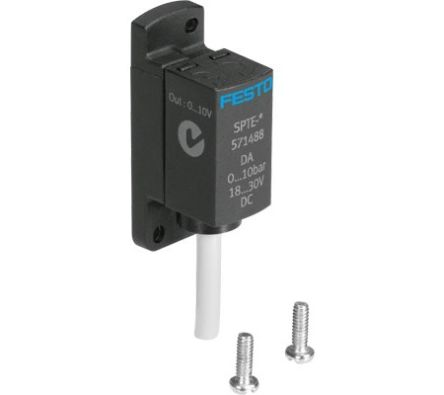
\includegraphics[width=0.4\linewidth, height=0.2\textwidth]{img/neumatico}
	\caption{}
	\label{fig:neumatico}
\end{figure} 

\textbf{Sensores piezoeléctricos: }
Los materiales piezoeléctricos presentan un fenómeno conocido como efecto piezoeléctrico. Este efecto ocurre cuando ciertos cristales elásticos asimétricos se deforman bajo la acción de una fuerza, generando un potencial eléctrico en su red cristalina. El proceso es reversible, lo que significa que al aplicar un voltaje entre las superficies del cristal, este experimentará un cambio en sus dimensiones físicas.

La magnitud y polaridad de las cargas inducidas dependen directamente de la intensidad y dirección de la fuerza aplicada. Algunos materiales piezoeléctricos comunes son el cuarzo, la turmalina y la sal de Rochelle. Los sensores piezoeléctricos permiten medir fuerzas en un rango de 1 a 20 kN, con una proporción de 2105. Debido a sus características, estos sensores son ideales para detectar cambios instantáneos en la fuerza, es decir, medir fuerzas dinámicas.

\begin{figure}[h]
	\centering
	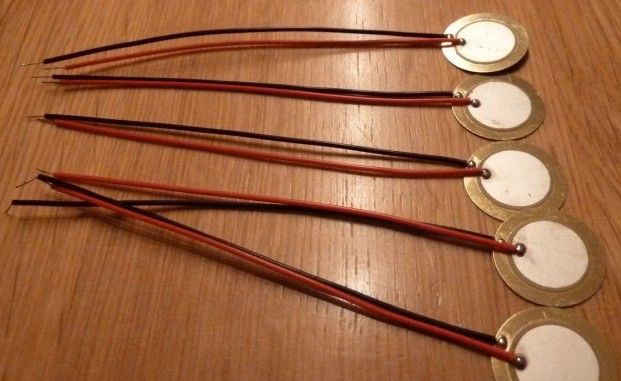
\includegraphics[width=0.4\linewidth, height=0.2\textwidth]{img/piezoele}
	\caption{}
	\label{fig:piezoele}
\end{figure} 

\textbf{Transductores de presión: }
Es un dispositivo que convierte la presión en una señal de salida eléctrica, esta puede ser digital o analógica y es utilizada por otros dispositivos como controladores, alarmas y otros sistemas de circuito cerrado. Estos dispositivos son cruciales para garantizar la seguridad y eficiencia en los sistemas al proporcionar datos de presión precisos. 



\begin{figure}[h]
	\centering
	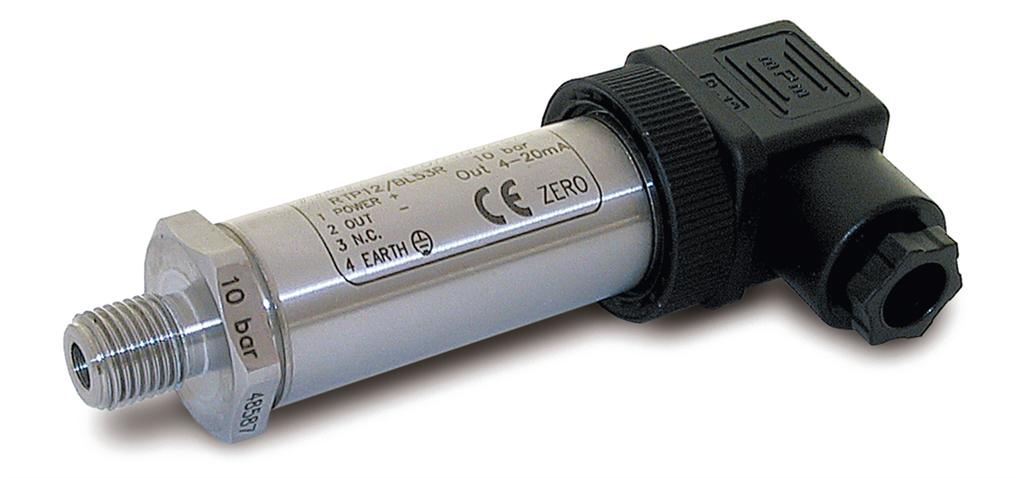
\includegraphics[width=0.4\linewidth, height=0.2\textwidth]{img/transductorpresion}
	\caption{}
	\label{fig:transductorpresion}
\end{figure} 

\textbf{Tipo sin contacto }

\textbf{Sensores de proximidad: }
Existen dos tipos de sensores de proximidad : inductivo y capacitivo. Los sensores de proximidad inductivos se usan en lugar de interruptores de límite para la detección sin contacto de objetos metálicos. Los sensores de proximidad capacitivos se usan sobre la misma base que los sensores de proximidad inductivos, pero también pueden detectar objetos no metálicos.



\begin{figure}[h]
	\centering
	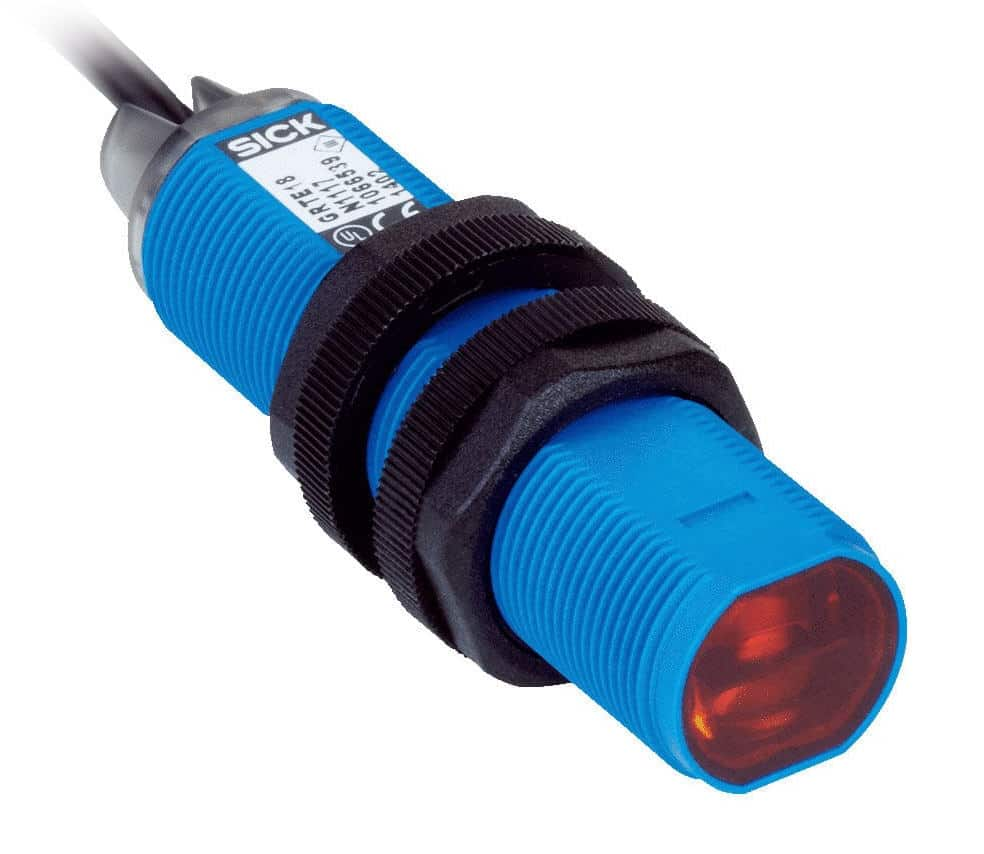
\includegraphics[width=0.4\linewidth, height=0.2\textwidth]{img/proximidad}
	\caption{}
	\label{fig:proximidad}
\end{figure} 

\textbf{Sensores de Efecto Hall: }
Un sensor de efecto Hall aprovecha, como su nombre indica, el efecto Hall, que puede producirse en un metal o en un semiconductor. Este efecto se basa en la interacción básica entre un electrón y un campo magnético. Cuando se aplica a semiconductores, el efecto Hall crea un interruptor digital que produce una muy eficiente señal de onda cuadrada de encendido-apagado. Perturbar la ventana entre el campo magnético y el chip de silicio produce una salida igual a cero.



\begin{figure}[h]
	\centering
	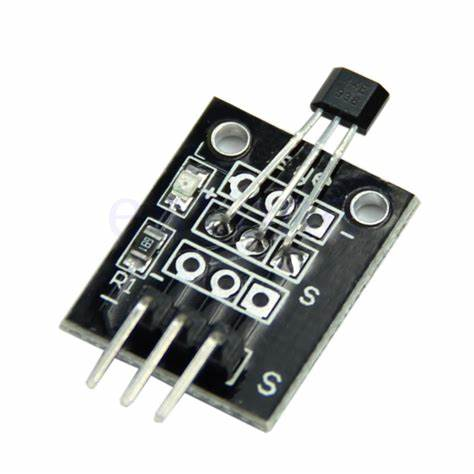
\includegraphics[width=0.4\linewidth, height=0.2\textwidth]{img/HALL}
	\caption{}
	\label{fig:HALL}
\end{figure} 

\textbf{Sensores de microondas: }
Son sensores que utilizan la frecuencia de microondas para detectar el movimiento en una zona mediante la emisión de impulsos de microondas y la posterior medición del reflejo de un objeto en movimiento. Funcionan según el principio del efecto Doppler. Cuando la frecuencia de microondas emitida encuentra un objeto en movimiento en su campo de detección, la frecuencia de retorno se altera, indicando así el movimiento.

\begin{figure}[h]
	\centering
	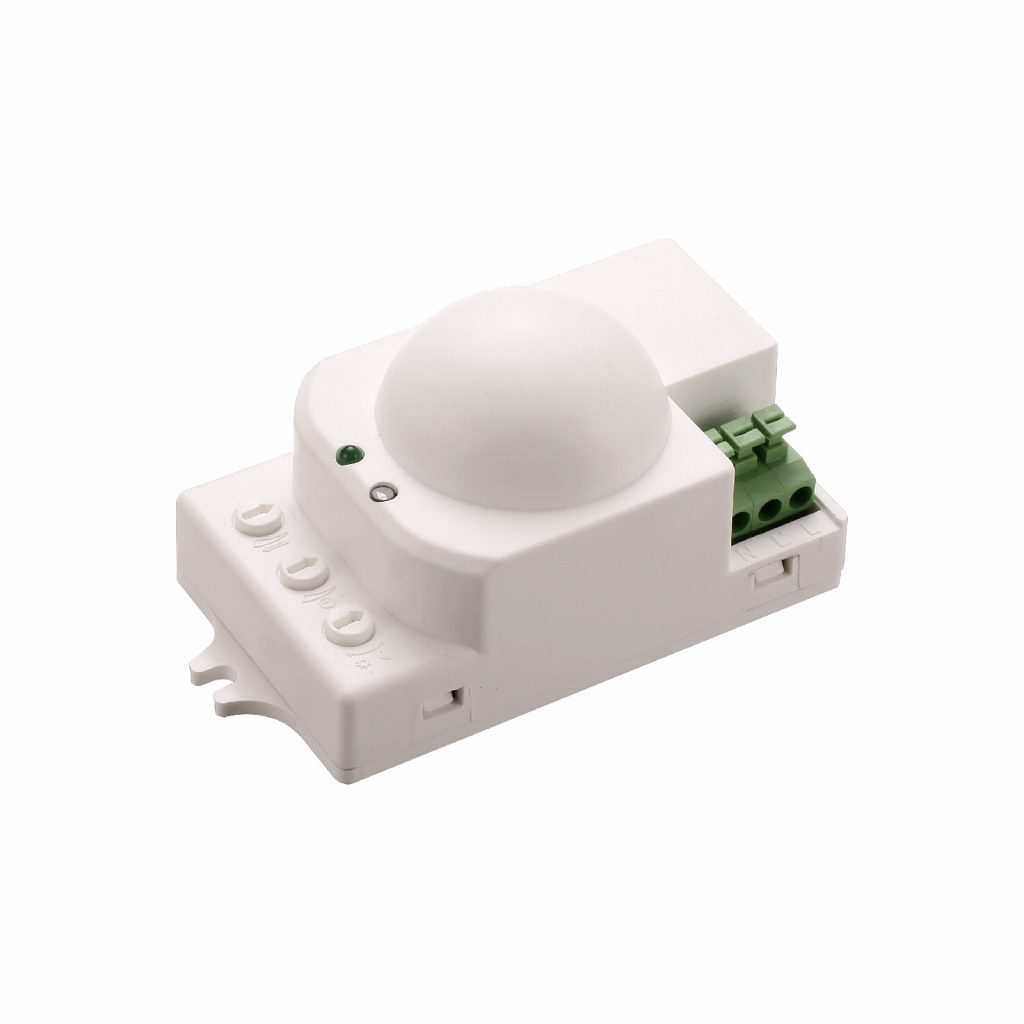
\includegraphics[width=0.4\linewidth, height=0.2\textwidth]{img/microondas}
	\caption{}
	\label{fig:microondas}
\end{figure} 

\textbf{Sensores ultrasónicos: }
Son sensores los cuales miden la distancia mediante el uso de ondas ultrasónicas. Está formado por un cabezal el cual emite una onda ultrasónica y recibe la onda reflejada que retorna desde el objeto. Este tipo de sensores miden la distancia al objeto  contando el tiempo entre la emisión y la recepción. 


\begin{figure}[h]
	\centering
	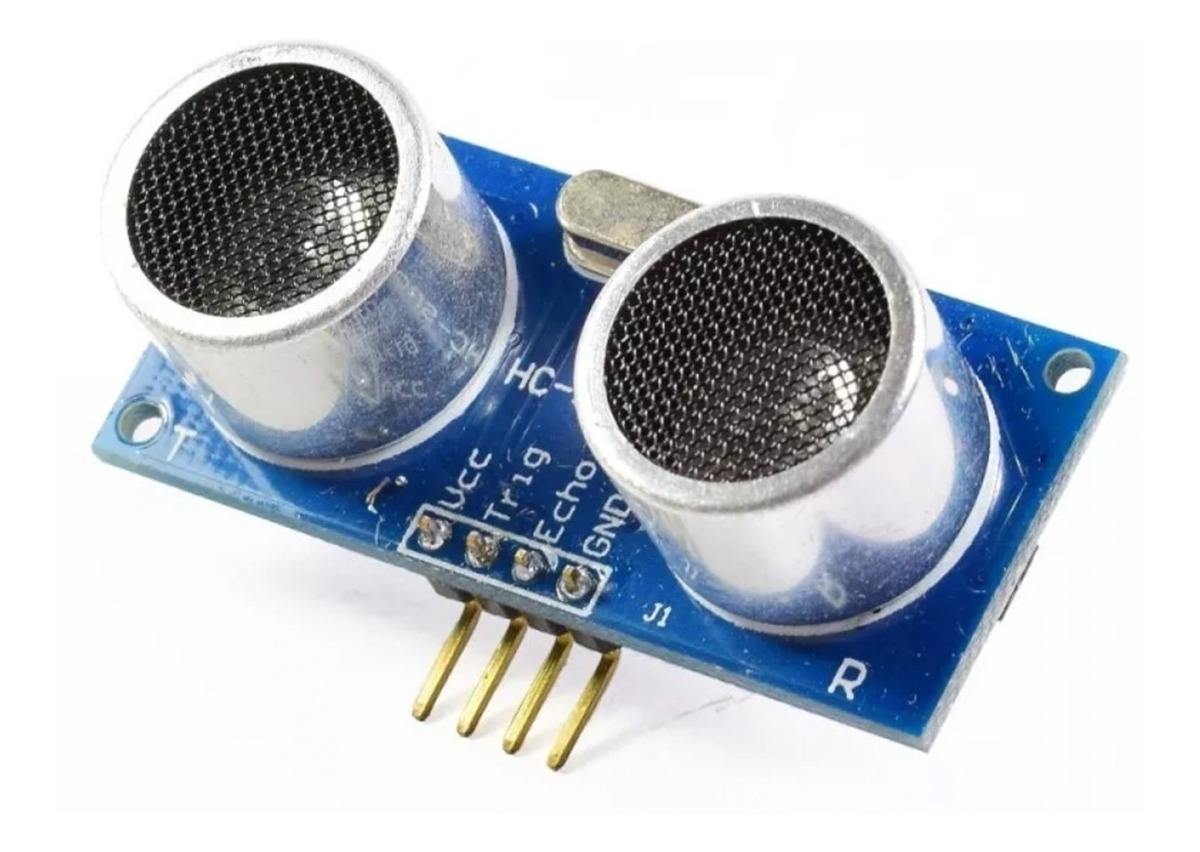
\includegraphics[width=0.4\linewidth, height=0.2\textwidth]{img/ultrasonido}
	\caption{}
	\label{fig:ultrasonido}
\end{figure} 

\textbf{Sensores Láser: }
Este tipo de sensores utiliza un “laser” para lograr emitir luz en una línea recta. Su punto de haz visible hace que su alineación y posicionamiento sean sencillos. Este haz de luz es emitido desde el elemento emisor de luz en el transmisor y es recibido por el elemento de recepción de luz en el receptor. \\\\\\\\\
\begin{figure}[h]
	\centering
	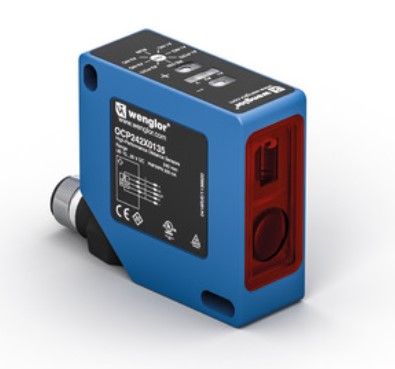
\includegraphics[width=0.4\linewidth, height=0.2\textwidth]{img/laser}
	\caption{}
	\label{fig:laser}
\end{figure} 




\textbf{Sensor de visión: }
Estos sensores son un tipo de solución de visión artificial los cuales utilizan imágenes capturadas por una cámara para determinar la presencia, orientación y  precisión de las piezas. Estos sensores se diferencian de los “sistemas” de inspección de imagen, en que la cámara, la luz y el controlador están contenidos en una sola unidad, lo que simplifica la construcción y operación de la misma.

\begin{figure}[h]
	\centering
	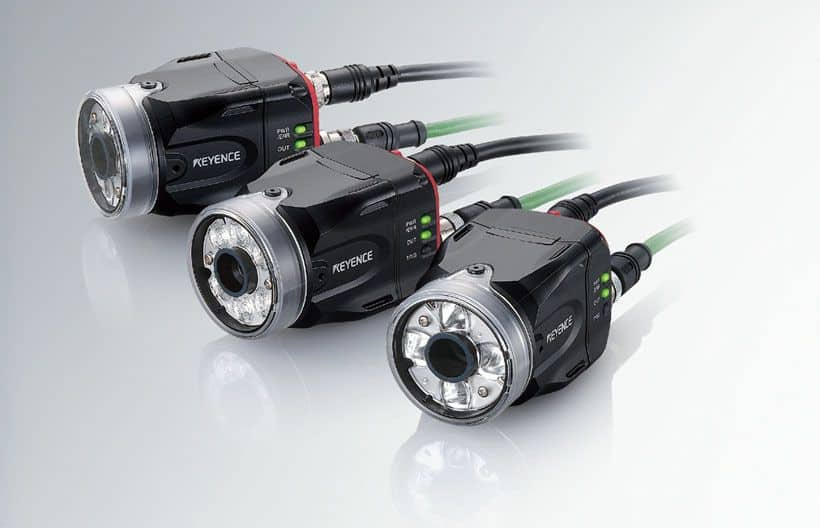
\includegraphics[width=0.4\linewidth, height=0.2\textwidth]{img/vision}
	\caption{}
	\label{fig:vision}
\end{figure} 

\section{Adicionales}
\textbf{Giroscopio:}
Este tipo de sensores utiliza un “laser” para lograr emitir luz en una línea recta. Su punto de haz visible hace que su alineación y posicionamiento sean sencillos. Este haz de luz es emitido desde el elemento emisor de luz en el transmisor y es recibido por el elemento de recepción de luz en el receptor. 
\vspace{10pt}  % Espacio de 10 puntos


\textbf{Acelerómetro:}
Un acelerómetro mide la aceleración a través del cambio en la capacitancia. Su estructura incluye una masa conectada a un resorte, permitiendo que se desplace en una dirección específica dentro de un marco con placas fijas. Cuando se aplica una aceleración, la masa se mueve, lo que modifica la capacitancia entre las placas y la masa. Este cambio es medido y procesado para determinar el valor de la aceleración correspondiente.
\vspace{10pt}  % Espacio de 10 puntos

\textbf{Magnetómetro:}
El magnetómetro detecta el campo magnético terrestre utilizando principalmente el efecto Hall o, en menor medida, el efecto magnetorresistivo. En la mayoría de los sensores del mercado, el efecto Hall funciona de la siguiente manera: si se aplica una corriente a través de una placa conductora, los electrones fluyen en línea recta. Sin embargo, la presencia de un campo magnético altera esta trayectoria, desviando los electrones hacia un lado de la placa y generando una diferencia de voltaje proporcional a la intensidad del campo. Por otro lado, los sensores que emplean el efecto magnetorresistivo utilizan materiales sensibles al magnetismo, como aleaciones de hierro y níquel. Cuando estos materiales son expuestos a un campo magnético, su resistencia eléctrica varía, permitiendo la medición del campo.
\vspace{10pt}  % Espacio de 10 puntos



\textbf{LiDAR:}
La tecnología LiDAR se emplea para crear mapas topográficos detallados y modelos 3D precisos, esenciales para la navegación de vehículos autónomos en entornos dinámicos. También se utiliza en la evaluación de riesgos naturales, como flujos de lava, deslizamientos de tierra, tsunamis e inundaciones.
Un sistema LiDAR típico consta de varios componentes:
Un escáner láser que emite pulsos de luz láser en el espectro casi infrarrojo.
Un sensor LiDAR que detecta y captura los pulsos reflejados.
Un procesador que calcula el tiempo y la distancia para construir la nube de puntos LiDAR resultante.
Para lograr una medición precisa, el sistema también incorpora componentes adicionales como electrónica de cronometraje, una unidad de medición inercial (IMU) y un GPS.
